% Toolbar icon: inspect — a viewfinder/reticle with a center dot (click a
% node/element to probe its data — distinct from find's magnifying glass,
% which locates a KNOWN id rather than picking one off the mesh).
% NOTE: the committed svg-ui/inspect.svg was hand-authored to the same
% drawing (no LaTeX toolchain available); regenerating via `make ui` replaces
% it with the pdftocairo rendering of this source — same glyph either way.
\documentclass[tikz,border=2mm]{standalone}
\usetikzlibrary{arrows.meta,calc}
\begin{document}
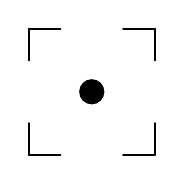
\begin{tikzpicture}[line width=1.3pt, line cap=round, line join=round, x=1mm,y=1mm]
  \foreach \x/\y/\dx/\dy in {-8/8/0/-4, -8/8/4/0, 8/8/0/-4, 8/8/-4/0, 8/-8/0/4, 8/-8/-4/0, -8/-8/0/4, -8/-8/4/0} {
    \draw[thick] (\x,\y) -- ($(\x,\y)+(\dx,\dy)$);
  }
  \fill (0,0) circle (1.6);                              % center dot
\end{tikzpicture}
\end{document}
